\section{Design Overview}
\label{s:design}
%
\begin{figure}[t]
\centering
    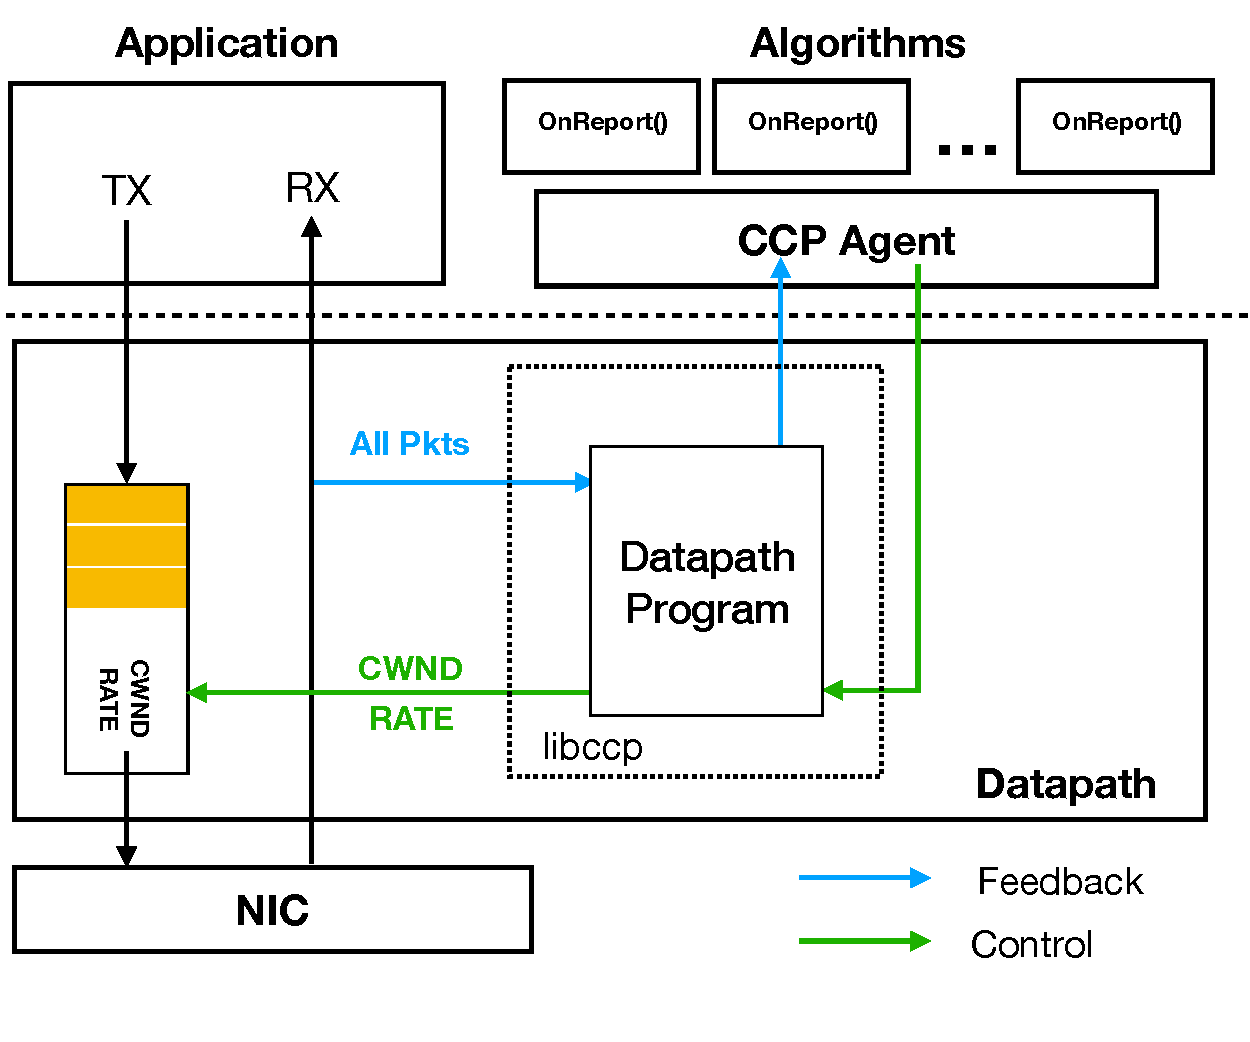
\includegraphics[width=\columnwidth]{img/ccp_design_sigcomm}
    \caption{Congestion control algorithms in CCP are distinct from the application and datapath.
    Users specify control patterns to set the congestion window or rate,
    and fold functions to define how to summarize datapath messages into reports processed in CCP.}\label{fig:design}
\end{figure}
%
Our design restructures congestion control by separating it into two distinct components: an off-datapath agent (CCP) and a set of interfaces that the datapath must provide. The CCP agent provides the execution environment for user-specified congestion control algorithms. It receives data about congestion signals from the datapath and invokes the algorithm's code that uses this data. The datapath is responsible for processing feedback (e.g., TCP or QUIC ACKs) from the receiver to provide congestion signals for the algorithms that run in CCP. The datapath also provides interfaces for CCP algorithms to set the congestion window and pacing rate, and express control patterns; these patterns can control transmission times and specify the times at which congestion signals are delivered to CCP.

\subsection{CCP-Datapath Isolation}

Should CCP run in the same address space as the datapath or not? There are some trade-offs involved in this decision. On the plus side, if run in the same address space, then information could be exchanged between them nearly instantaneously at high bandwidth, and a congestion signal could be sent from the datapath to CCP every time feedback from the receiver arrives. But there are two drawbacks to this approach:

\paragrapha{Safety} Bugs in CCP or in the algorithm's code could cause datapath crashes, or cause vulnerabilities that trigger privilege escalation attacks on kernel datapaths. 
To cope, at a minimum, we would have to enforce restrictions on the kernel functions that CCP can use, and adopt methods from recent research on kernel software fault isolation (LXFI~\cite{lxfi}). 
This approach will have a non-trivial performance impact, quite likely defeating the purpose of running CCP in the same address space as the datapath. 
This approach also requires a careful annotation of kernel functions, and the specification of principals and kernel API integrity rules, a challenging task because the network stack has a large number of functions with subtle behaviors.
    
\paragrapha{Flexibility} In the future, we anticipate running CCP on a different machine from the sender to centralize congestion control policies across groups of hosts. 
The same-address-space CCP would require a substantial re-design for this mode of operation.

\begin{table}[]
    \centering
    \begin{tabular}{c|c|c}
        Implementation & Reporting Interval & Mean Throughput \\
        \hline
        Kernel & - & $43$ Gbit/s \\
        CCP & Per ACK & $29$ Gbit/s \\
        CCP & Per $10$ ms & $41$ Gbit/s \\
    \end{tabular}
    \caption{Single-flow throughput for different reporting intervals between the Linux TCP datapath and user-space CCP, compared to kernel TCP throughput. Per-ACK feedback (0 $\mu$s interval) reduces throughput by 32\%, a significant amount, while using a $10$ ms reporting interval achieves almost identical throughput to the kernel. Results as the number of flows  increases are in \S\ref{sec:eval:whyfold}.}\label{fig:perf:interval}
\end{table}
%\begin{figure}[t]
%    \centering
%    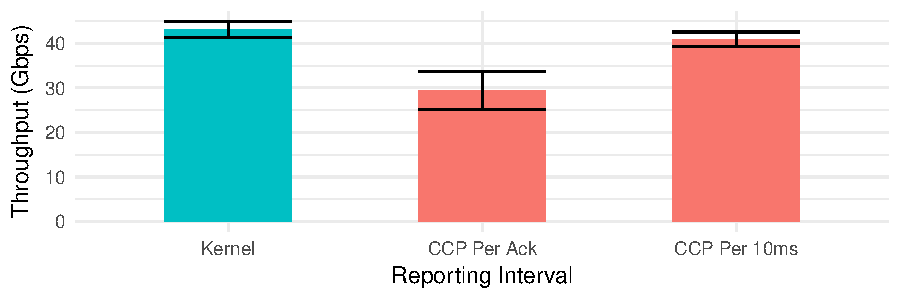
\includegraphics[width=\columnwidth]{img/max-throughput}
%    \caption{Throughput for different reporting intervals between the Linux TCP datapath and user-space CCP, compared to kernel TCP throughput. Per-ACK feedback (0 $\mu$s interval) reduces throughput by 32\%, a significant amount.}\label{fig:perf:interval}
%\end{figure}

\smallskip

Our design supports both modes, but we focus on how to achieve high performance and fidelity when CCP is in a different address space, including the important case when the datapath is kernel TCP and CCP is in user space.

When CCP is in a different address space, providing per-ACK notifications from the datapath to CCP incurs high overhead, as shown in Figure~\ref{fig:perf:interval}. This experiment shows that for a saturating iperf connection over a loopback interface, the Linux kernel TCP on this machine  (with 4 2.8 Ghz cores) achieves $45$ Gbit/s running Reno, whereas per-ACK reporting from the kernel datapath to CCP running Reno achieves only 68\% of the throughput of the kernel. 
One way to improve performance is to increase the time between reports sent to CCP. The ``Per 10 ms'' bar shows that a less frequent reporting period achieves close to the kernel's throughput. 
%\ma{are we going to add more reporting periods (other than 10 ms) to the figure?}

\if 0
One could combat this issue by moving CCP closer to the datapath; \ie either by placing them in the same address space or perhaps by using more efficient IPC mechanisms. Indeed, the design of CCP allows for such solutions. 

\fi

Given that CCP should report measurements only infrequently, a key question is how best to {\em summarize} congestion signals on the datapath so that CCP algorithms can achieve high fidelity compared to a baseline that implements the algorithm within the datapath. 
Although we are optimistic that a good design can achieve high fidelity because the natural time-scale for end-to-end congestion control is the RTT between sender and receiver, achieving it requires a careful design of the information channel between datapath and CCP. 

In \S\ref{sec:eval:fidelity} we show that using a larger reporting period does not affect the fidelity of CCP algorithm implementations relative to native datapath ones. 

\if 0
As a result, we anticipate that developers will choose a reporting interval for their algorithms that meet the needs of their specific deployment. 
\fi

\subsection{Exercising Control over Datapath Functions}

% CCP algorithms specify datapath behavior using two mechanisms: {\em fold functions} and {\em control patterns},  whose directives are used by the datapath to summarize congestion signals sent to CCP, and {\em send patterns}, which control packet transmissions on the datapath. 

Congestion-control algorithms written in CCP are not tied to the traditional ``ACK clock'', but rather operate on summaries that encapsulate observations over multiple ACKs received by the datapath sender.
CCP algorithms specify datapath behavior using two mechanisms: {\em fold functions} and {\em control patterns}, whose directives are interpreted by the datapath to summarize congestion signals sent to CCP and control packet transmissions on the datapath, respectively. 

\paragrapha{Congestion signals and fold functions} All CCP-compatible datapaths should export a well-defined set of congestion signals (Table~\ref{tab:datapath:signals}). There are two kinds of congestion signals: \texttt{Ack} signals, which are computed directly on each ACK (e.g., bytes acked in order, bytes acked out of order, RTT sample, etc.) and \texttt{Flow} signals, which are statistics maintained for the flow (e.g., outgoing and incoming rates). Most of these signals are updated on the arrival of an ACK; the exceptions are: \texttt{was\_timeout} and \texttt{lost\_pkts\_sample} updated on a timeout; and \texttt{bytes\_in\_flight} and \texttt{packets\_in\_flight} updated on packet transmissions.

% update others might update on a timeout or at other times. \ma{this is vague. what `other times'?}

\begin{table}
    \centering
    \footnotesize
    \begin{tabular}{p{0.4\columnwidth}p{0.6\columnwidth}}
      \textbf{Signal} & \textbf{Definition} \\
      \hline
        \texttt{bytes\_acked}, \texttt{packets\_acked} & In-order acknowledged \\
        \texttt{bytes\_misordered}, \texttt{packets\_misordered} & Out-of-order acknowledged \\
        \texttt{ecn\_bytes}, \texttt{ecn\_packets} & ECN-marked \\
        \texttt{lost\_pkts\_sample} & Number of lost packets \\
        \texttt{was\_timeout} & Did a timeout occur? \\
        \texttt{rtt\_sample\_us} & A recent sample RTT \\
        \texttt{rate\_outgoing} & Outgoing sending rate \\
        \texttt{rate\_incoming} & Receiver-side receiving rate  \\
        \texttt{bytes\_in\_flight}, \texttt{packets\_in\_flight} & Sent but not yet acknowledged \\
        \texttt{now} & Datapath time (e.g., Linux \texttt{jiffies})\\
    \end{tabular}
    \vspace{0.075in}
    \caption{Congestion signals that datapaths should report.}\label{tab:datapath:signals}
\end{table}

CCP may read but not write these signals. The only way to gain access to them is via a fold function, which specifies how the datapath should summarize the congestion signals in a single reporting period. 
%For example, a CCP algorithm may ask to receive the sum of the bytes acknowledged in order, the moving average of the RTT samples, and the latest value of the flow's outgoing rate in a reporting period. 

%CCP is unaware of how a datapath computes these signals; for example, it does not know which variables the datapath uses to compute the signals. A CCP algorithm, however, specifies how it wants the datapath to summarize each signal over a reporting period using a small language. 

%

\begin{table}
    \centering
    \footnotesize
    \begin{tabular}{p{0.4\columnwidth}p{0.6\columnwidth}}
      \textbf{Class} & \textbf{Operations} \\
      \hline
        Arithmetic & $+, -, *,$~/$,$ EWMA \\
        Comparison & $==, <, >$ \\
        Conditionals & If (branching) \\
        Assignment & $:=$ \\
    \end{tabular}
    %\vspace{0.075in}
    \caption{Fold function operators that a datapath must support.}\label{tab:datapath:operators}
\end{table}


Fold functions express simple operations over the congestion signal primitives. Table~\ref{tab:datapath:operators} contains the operations each datapath should be able to compute. A CCP algorithm expresses fold functions in a small, restrictive domain-specific language. Each datapath must support this language. For software datapaths, we have developed \texttt{libccp}, a library that provides a reference implementation of fold function computations in this language and other features common to all datapaths (see \S\ref{s:datapath:libccp}). 

The fold function defines a structure called \texttt{Summary}. This structure is maintained by the datapath and encapsulates all measurements reported to CCP by the datapath. The CCP algorithm specifies the fields of the \texttt{Summary} structure in the fold function and how to compute each field from congestion signals. The algorithm may define as many fields as it wants in the \texttt{Summary} structure. The datapath writes the values of these fields using the logic supplied by the CCP algorithm.

The following fold function shows an example of how to request the number of bytes delivered in order within the reporting period. The sender's datapath runs this function on each received ACK, \texttt{A}:

\begin{minted}{lisp}
  (def (Summary.acked 0))
  (:= Summary.acked
    (+ Summary.acked A.bytes_acked))
\end{minted}

%The fold function defines a \texttt{Summary} signal, which is the third type of signal maintained by the datapath. 
%Unlike \texttt{Ack} and \texttt{Flow} signals, which are read-only, \texttt{Summary} signals are writeable by the CCP algorithm. 

In the example above, the fold function defines a field, \texttt{Summary.acked}, and specifies that on each invocation (typically every received ACK), it should be incremented by the number of in-order bytes observed since the last invocation. After delivering the summary, the datapath resets each reported \texttt{Summary} field to the specified initial value.

%We specify the complete list of available signals and built-in operations on them in \S\ref{s:datapath:fold}.

\paragrapha{Control patterns} CCP algorithms can specify the congestion window or pacing rate using simple functions supported by the datapath. These can be set to either absolute values or relative to current values. The algorithms can also specify timing patterns according to which summary reports from fold functions and window/rate settings are executed by the datapath. 
The ability to specify timing patterns is useful for two reasons. First, algorithms may wish to specify patterns of sending; BBR~\cite{bbr}, for example, sends pulses of different magnitudes for specific time durations. Second, algorithms may wish to specify the precise intervals over which congestion signals should be gathered and reported (e.g., once every half-RTT).

\begin{minted}{rust}
SetCwndAbs(...) => WaitRtts(0.5) => Report()
\end{minted}

Control patterns use \texttt{=>} to specify that the directive on the right should happen after the one on the left. This example pattern uses the \texttt{WaitRtts()} directive to specify that the datapath should set the congestion window to the specified value, wait for a half-RTT, and then report a summary to CCP. After this report, the pattern will reset Summary state and loop back to \texttt{SetCwndAbs()}.

%We study this behavior with several experiments in \S\ref{s:eval:fidelity}.

Figure~\ref{fig:design} shows the architecture of a CCP-enabled sender, highlighting how the components we have discussed in this section fit together. 


\if 0
    \2 For example, many datapaths maintain notions of the most recent cumulative acknowledgement received.
        \3 TCP and mTCP call this \texttt{snd\_una}, and QUIC calls it \an{foo}.
        \3 CCP calls the delta of this quantity corresponding to each invocation \texttt{bytes\_acked}.
    \2 The datapath also must implement the measurements specified by the fold function, and enforce the rates specified by the send pattern.
        \3 We describe our implementation of a reference library implementing these features, libccp, in .
        
\fi

%\1 Design. What is our proposed design? (3-4 pages)
%    \2 CCP: a congestion control plane is a module in which the logic for congestion control in its various forms resides.
%    \2 A ``datapath'' is an entity which:
%        \3 transfers data from applications to the wire
%        \3 includes the transport layer and below.
%        \3 complies with the libccp interface, which is explained below.
%    \2 Where should CCP be: In-kernel or userspace?
%        \3 benefits of in-kernel
%            \4 usable across all applications
%            \4 ``safe''?
%            \4 high performance
%        \3 disadvantages of in-kernel
%            \4 usage with kernel-bypass datapaths is awkward
%            \4 programming is more difficult
%            \4 trusted computing base size is large
%        \3 we conclude CCP should be in userspace
%    \2 CCP Design
%        \3 Two components: algorithm API to implement congestion control schemes, and datapath API to support CCP
%        \3 algorithm API
%            \4 Event Handlers
%            \4 OnCreate: a new flow has begun
%            \4 OnMeasurement: a congestion event has occurred. The measurements returned and when this even is triggered is governed by the user-provided fold function and send pattern
%            \4 send patterns: user specifies a sequence of states the datapath should transition through, synced to the ACK clock.
%            \4 fold function: user specifies a program in a \emph{constrained, domain specific language with a lisp-like syntax} which is run upon every packet. Program decides what measurements to store, and whether to bypass the send pattern's default measurement period and notify CCP immediately. fold function can also optionally set the congestion window.
%            \4 discuss tradeoffs of setting cwnd in fold function vs in CCP (more vs less control, more vs less reactiveness)
%        \3 datapath API (libccp): datapath implements the libccp interface by providing function pointers
%            \4 primitives: datapath returns a list of congestion control primitives for the fold function to operate over: ACK, Losses, ECN?, RTT, Rates
%            \4 maintain rate, cwnd
%            \4 IPC mechanism: datapath provides a way to send a message to CCP, and calls a libccp callback upon a CCP response.
%            \4 datapath calls libccp\_invoke() upon every packet (or atomic congestion control timestep) to advance libccp's state machine
%        \3 why have a query processor?
%        \3 fold function primitives: data model
%            \4 ``streaming tuple'': full generality (will this be ready???)
%            \4 higher-level datapath-provided primitives
%\1 Implementation
%    \2 CCP implementation
%        \3 We implemented a CCP in rust, portus
%        \3 library for congestion control binaries to use
%            \4 implements serialization/IPC and language support for communicating with datapath libccp
%    \2 libccp implementation
%        \3 describe fold functions implementation
%            \4 compilation to datapath-friendly instructions. like eBPF, but specialized for congestion control information, and not just in the kernel. It was easier to add libccp support to the kernel than make eBPF work for general datapaths.
%            \4 state machine with registers to run datapath measurement instructions